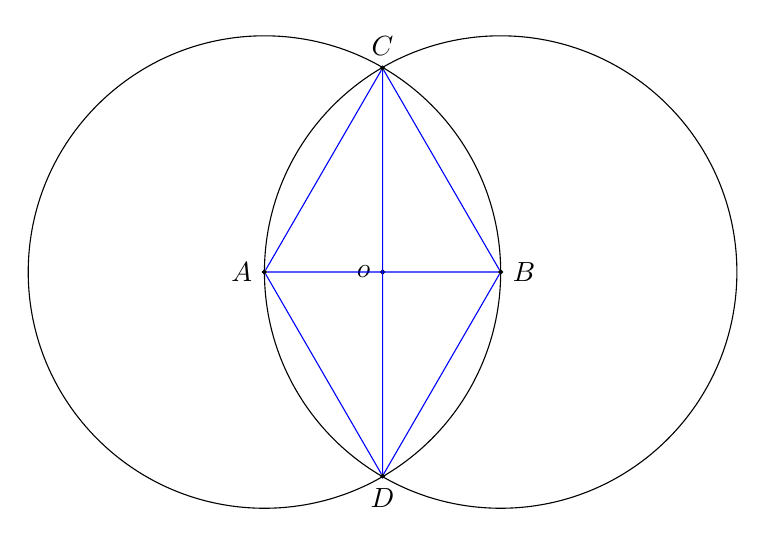
\begin{tikzpicture}
[scale=1,>=stealth,point/.style={draw,circle,fill = black,inner sep=0.5pt},]
%Inradius
\def\r{3} 
\node (A) at (0,0)[point,label=left:$A$] {};
\def\s{3} 
\node (B) at (3,0)[point,label=right:$B$] {};

%Drawing circle
\color{black}
\draw (A) circle (\r);
\draw (B) circle (\s);

%intersecting points
\def\a{1.5}
\def\b{2.59}
\color{black}
\node (C) at (\a,\b)[point,label=above:$C$] {};
\node (D) at (\a,-\b)[point,label=below:$D$] {};
\node (o) at (\a,0)[point,label=left:$o$] {};

%Drawing Rhombus
\color{blue}
\draw (A) -- node[left] {$\textrm{}$} (B) -- node[below] {$\textrm{}$} (C) -- node[right,,xshift=2mm] {$\textrm{}$} (A)-- node[below] {$\textrm{}$} (D)-- node[below] {$\textrm{}$} (B) (D)-- node[below] {$\textrm{}$} (C);
%Drawing the angles
\tkzMarkRightAngle[fill=black!20,size=.3](C,o,B)
\tkzMarkRightAngle[fill=black!20,size=.3](C,o,A)
\tkzMarkRightAngle[fill=black!20,size=.3](D,o,B)
\tkzMarkRightAngle[fill=black!20,size=.3](D,o,A)
\end{tikzpicture}